\section{API's development}
\label{section:API}
The work here focused on the implementation of SISYPHE's API and its coupling to TELEMAC2D's already available API via FORTRAN modules. The API's main goal is to have control on a simulation while running a case. For example, it must allow the user to stop the simulation at any time step, retrieve some variables values and change them if necessary. SISYPHE's API is contained in the source folder of the TMS, as shown in Figure \ref{fig:API_sources}, and can therefore call all SISYPHE's subroutines to conduct morphodynamic simulations.
\begin{figure}[h!]
    \centering
    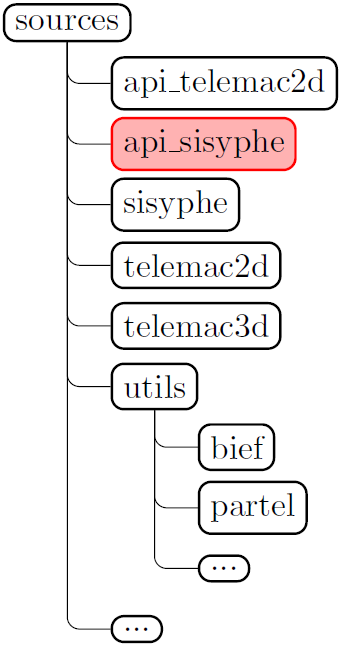
\includegraphics[trim={0 0 0 0},clip,scale=0.3]{Images/API_sources}
    \caption{Extract of TELEMAC-MASCARET sources folders}
    \label{fig:API_sources}
    \vspace{-0.5cm}
\end{figure}

In order to make this possible, a FORTRAN structure called instance was developed in the API. It contains a list of variables declared as pointers (memory addresses \cite{bib10}) that are pointing to SISYPHE's variables. This gives direct access to the physical memory of variables, and allows therefore to retrieve their values, and modify them. Furthermore, modifications have been made in SISYPHE's main subroutines to make morphodynamic cases execution possible time step by time step. Finally, parallel runs have also been treated.

In addition to this, to make running coupled cases via the API possible, a communication interface is developed in FORTRAN. This interface contains communication subroutines that send TELEMAC2D's variables to SISYPHE and vice-versa. It also contains subroutines that manage coupled cases and take into consideration the coupling period. 

A number of modifications in TELEMAC2D and SISYPHE sources were necessary. These modifications, along with the API and the coupling developments, were validated using three different compilers (NAG, IFORT, GFORTRAN), on classical SISYPHE cases and coupled TELEMAC2D-SISYPHE cases, available in the system.

\textcolor{red}{Parler du wrapping Python}

blabla

\textcolor{red}{décrir le lien API-calage et API-incertitudes}
